\title{ 10. Kombinatorika}
\author{Marek Fuchs (Oliver Hadraba)}
\date{26.4.2025}

\maketitle



\section{Kombinatorika}
    
     \subsection{Faktoriál}
     Faktoriál čísla $n$ je roven součinu všech přirozených čísel $N$ $(1;2;3;..)$, která jsou menší nebo rovna číslu $n$.\\
     Faktoriál zapisujeme pomocí vykřičníku $\rightarrow{n!}$\\
    Například: $5! = 5\cdot4\cdot3\cdot2\cdot1=120$
     
     \subsection{Variace}
     Variace k-té třídy z $n$ prvků je každá uspořádaná k-tice vytvořená z celkového počtu $n$ prvků, přičemž při výběru záleží na pořadí jednotlivých prvků.
     \begin{itemize}
         \item Bez opakování
         $$
         V_k (n)=\frac{n!}{(n-k)!}
         $$
         \item S opakováním
         $$
         V_k (n)=n^k
         $$
     \end{itemize}
Například: Vybíráme 4 studenty z 25 na zkoušení a záleží jim na tom, kolikátí budou vybráni, aby se mohli učit co nejdéle. V tomto případě záleží na pořadí a proto pro výpočet počtu možností použijeme variace. 

     \subsection{Permutace}
     Kolika způsoby lze uspořádat všechny $n$ prvky.\\
     Permutace je zvláštní případ variace, kde $k=n$. To znamená, že ze zadaných prvků postupně vybereme všechny. Každá permutace tedy odpovídá nějakému pořadí zadaných prvků: každý prvek se v pořadí musí objevit, ale žádný tam nemůže být dvakrát. Permutace z $n$ prvků je každá n-členná variace z těchto prvků.
     $$
     P(n)=n!
     $$
     $$
     P(n)=n \cdot(n-1)\cdot(n-2) \ ...2\cdot1=n!
     $$
     Případ, kdy zkoušíme všechny studenty.
     \subsection{Kombinace}
     Kombinace je neuspořádaná k-tice vytvořená z celkového počtu $n$ prvků, přičemž nezáleží na pořadí vybraných prvků.
     \begin{itemize}
         \item Bez opakování
         $$
         C_k (n)= {n \choose k}=\frac{n!}{k!(n-k)!}
         $$
         Využíváme například, pokud vybíráme z 6 kluků 3, kteří budou současně zametat (nezáleží na pořadí v kterém budou vybráni)
         \item S opakováním
         $$
         C_k(n)= {n+k-1 \choose k}
         $$
     \end{itemize}
     
     \subsection{Kombinační číslo}
     \textbf{Kombinační číslo}, označované jako $\binom{n}{k}$ (čteme: n nad k), udává počet způsobů, jak lze z množiny $n$ prvků vybrat právě $k$ prvků bez ohledu na pořadí.

Matematicky je definováno jako:

\[
\binom{n}{k} = \frac{n!}{k!(n-k)!}, \quad \text{pro } 0 \leq k \leq n
\]

kde $n!$ značí \textit{faktoriál} čísla $n$, tedy součin všech přirozených čísel od $1$ do $n$.

Pro $k > n$ platí:

\[
\binom{n}{k} = 0
\]
     \subsection{Binomická věta}
     Binomická věta říká, že:
     $$
        (a + b)^n = \sum_{k=0}^{n} \binom{n}{k} a^{n-k} b^k
     $$
     Znamená to, že výraz $(a + b)^n$ se rozepíše jako součet členů, ve kterých:

\begin{itemize}
  \item mocniny $a$ a $b$ se vždy doplňují do $n$,
  \item koeficienty jsou \textbf{binomické koeficienty}: 
  \[
  \binom{n}{k} = \frac{n!}{k!(n-k)!},
  \]
  \item index $k$ určuje, kolikrát se v daném členu vyskytuje $b$, a tedy i kolikrát $a$.
\end{itemize}

\subsubsection{Příklad pro $n = 3$}

\[
(a + b)^3 = \binom{3}{0}a^3b^0 + \binom{3}{1}a^2b^1 + \binom{3}{2}a^1b^2 + \binom{3}{3}a^0b^3
\]

\[
= 1 \cdot a^3 + 3 \cdot a^2b + 3 \cdot ab^2 + 1 \cdot b^3
\]

\[
= a^3 + 3a^2b + 3ab^2 + b^3
\]
\\
     Při řešení různých algebraických úloh potřebujeme občas umocnit dvojčlen $a+b$ na přirozené číslo $n$, tj. vypočítat $(a+b)^n$.\\
     Když chceme určit k-tý člen binomického rozvoje použijeme tento vzoreček:
     $$
     (a+b)^n={n \choose k-1}\cdot a^{n-(k-1)}\cdot b^{k-1}
     $$
     Příklad:\\
     Určete čtvrtý člen výrazu $(x+2)^{12}$
     $$
     (x+2)^{12}={12 \choose 3}\cdot x^9\cdot 2^3=220\cdot x^9 \cdot8=1760x^9
     $$
     \subsection{Pascalův trojúhelník}
     Je tvořen čísly a platí, že číslo, které se nachází pod jinými dvěma čísly, se rovná jejich součtu.\\
     \\

\begin{figure}[H]
        \centering
        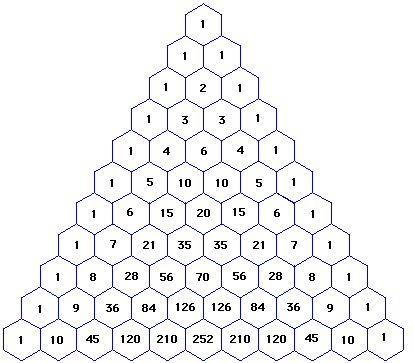
\includegraphics[width=0.4\linewidth]{img/21_pascaluvTrojuhelnik1_realny.jpg}
        \caption{Pascalův trojúhelník s přirozenými čísly} 
        \label{fig:enter-label}
    \end{figure}

\begin{figure}[H]
        \centering
        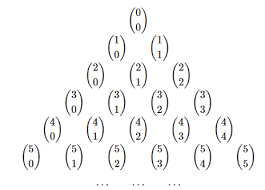
\includegraphics[width=0.4\linewidth]{img/21_paskal_kombinacni_cisla.png}
        \caption{Pascalův trojúhelník s kombinačními čísly} 
        \label{fig:enter-label}
    \end{figure}
    
     
\subsection{Výpočet rovnice}
Upravme výraz:
\[
\frac{1}{n!} - \frac{3}{(n+1)!}
\]

Společný jmenovatel je $(n+1)! = (n+1) \cdot n!$:

\[
= \frac{(1)(n+1) - 3}{(n+1)!} = \frac{n - 2}{(n+1)!}
\]

\subsection{Speciální případy kombinačních čísel}
     \begin{itemize}
         \item $k=0$
         $$
         {n \choose 0}=\frac{n!}{0!(n-0)!}=\frac{n!}{n!}=1
         $$
         \item $k=n$
         $$
         {n \choose n}=\frac{n!}{n!(n-n)!}=\frac{n!}{n!}=1
         $$
         \item $k=1$
         $$
         {n \choose 1}=\frac{n!}{1!(n-1)!}=n!
         $$
     \end{itemize}
     \subsection{Vlastnosti kombinačních čísel}
      \begin{itemize}
         \item Pro všechna celá nezáporná čísla $n$, $k$ platí $\rightarrow{k\leq n}$
         $$
         {n \choose n-k}={n \choose k}
         $$
         \item Důkaz:
         $$
         {n \choose n-k}=\frac{n!}{(n-k)![n-(n-k)]!}=\frac{n!}{k!(n-k)!}={n \choose k}
         $$
         \item Tato vlastnost popisuje jednoduchý fakt: Chceme li vybrat k-prvkovou podmnožinu n-prvkové množiny, zbyde vždy $n-k$ nevybraných prvků. Rozhodneme li se tedy vybrat $n-k$ prvků, které do hledaný podmnožiny nezařadíme, počet možností, jak je vybrat bude stejný jako při přímém výběru $k$.
     \end{itemize}
     